\documentclass{article}\usepackage[]{graphicx}\usepackage[]{color}
%% maxwidth is the original width if it is less than linewidth
%% otherwise use linewidth (to make sure the graphics do not exceed the margin)
\makeatletter
\def\maxwidth{ %
  \ifdim\Gin@nat@width>\linewidth
    \linewidth
  \else
    \Gin@nat@width
  \fi
}
\makeatother

\definecolor{fgcolor}{rgb}{0.345, 0.345, 0.345}
\newcommand{\hlnum}[1]{\textcolor[rgb]{0.686,0.059,0.569}{#1}}%
\newcommand{\hlstr}[1]{\textcolor[rgb]{0.192,0.494,0.8}{#1}}%
\newcommand{\hlcom}[1]{\textcolor[rgb]{0.678,0.584,0.686}{\textit{#1}}}%
\newcommand{\hlopt}[1]{\textcolor[rgb]{0,0,0}{#1}}%
\newcommand{\hlstd}[1]{\textcolor[rgb]{0.345,0.345,0.345}{#1}}%
\newcommand{\hlkwa}[1]{\textcolor[rgb]{0.161,0.373,0.58}{\textbf{#1}}}%
\newcommand{\hlkwb}[1]{\textcolor[rgb]{0.69,0.353,0.396}{#1}}%
\newcommand{\hlkwc}[1]{\textcolor[rgb]{0.333,0.667,0.333}{#1}}%
\newcommand{\hlkwd}[1]{\textcolor[rgb]{0.737,0.353,0.396}{\textbf{#1}}}%

\usepackage{framed}
\makeatletter
\newenvironment{kframe}{%
 \def\at@end@of@kframe{}%
 \ifinner\ifhmode%
  \def\at@end@of@kframe{\end{minipage}}%
  \begin{minipage}{\columnwidth}%
 \fi\fi%
 \def\FrameCommand##1{\hskip\@totalleftmargin \hskip-\fboxsep
 \colorbox{shadecolor}{##1}\hskip-\fboxsep
     % There is no \\@totalrightmargin, so:
     \hskip-\linewidth \hskip-\@totalleftmargin \hskip\columnwidth}%
 \MakeFramed {\advance\hsize-\width
   \@totalleftmargin\z@ \linewidth\hsize
   \@setminipage}}%
 {\par\unskip\endMakeFramed%
 \at@end@of@kframe}
\makeatother

\definecolor{shadecolor}{rgb}{.97, .97, .97}
\definecolor{messagecolor}{rgb}{0, 0, 0}
\definecolor{warningcolor}{rgb}{1, 0, 1}
\definecolor{errorcolor}{rgb}{1, 0, 0}
\newenvironment{knitrout}{}{} % an empty environment to be redefined in TeX

\usepackage{alltt}
\IfFileExists{upquote.sty}{\usepackage{upquote}}{}

\begin{document}

\begin{kframe}
\begin{alltt}
\hlkwd{library}\hlstd{(xtable)}
\hlstd{c} \hlkwb{<-} \hlkwd{xtable}\hlstd{(}\hlkwd{summary}\hlstd{(cars))}
\hlkwd{print}\hlstd{(c,} \hlkwc{type} \hlstd{=} \hlstr{"latex"}\hlstd{)}
\end{alltt}
\end{kframe}% latex table generated in R 3.0.2 by xtable 1.7-1 package
% Tue Dec 31 22:09:20 2013
\begin{table}[ht]
\centering
\begin{tabular}{rll}
  \hline
 &     speed &      dist \\ 
  \hline
1 & Min.   : 4.0   & Min.   :  2   \\ 
  2 & 1st Qu.:12.0   & 1st Qu.: 26   \\ 
  3 & Median :15.0   & Median : 36   \\ 
  4 & Mean   :15.4   & Mean   : 43   \\ 
  5 & 3rd Qu.:19.0   & 3rd Qu.: 56   \\ 
  6 & Max.   :25.0   & Max.   :120   \\ 
   \hline
\end{tabular}
\end{table}
\begin{kframe}\begin{alltt}
\hlkwd{plot}\hlstd{(cars)}
\end{alltt}
\end{kframe}
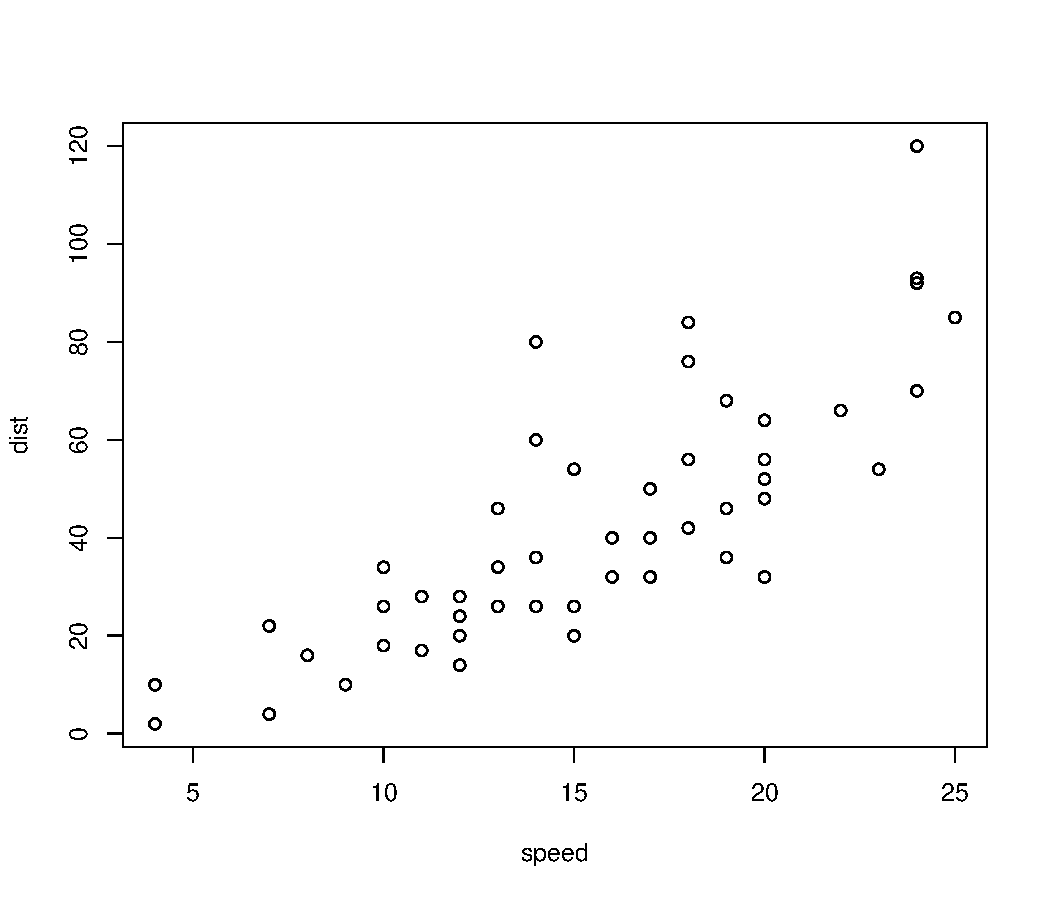
\includegraphics[width=\maxwidth]{figure/example} 



\centering
$\Gamma = \beta_0 + {\beta_1}^2 + \sum_{n=1}^{10}$

\end{document}
